\section{Appendix A. LLM Production Stages}

The initial set of failure modes were produced by examining each of the stages of benchmark production and both brainstorming a list of failure modes for each stage and capturing those failure mode mitigated by leading benchmarks.  LLM benchmarks are typically produced in an iterative manner as detailed in Figure \ref{fig:benchmark-production}. We briefly introduce these steps in turn below.  When scoring benchmark reliability, users needs to address and assess all stages of the benchmark's assembly. 

\begin{figure}[h!]
  \centering
  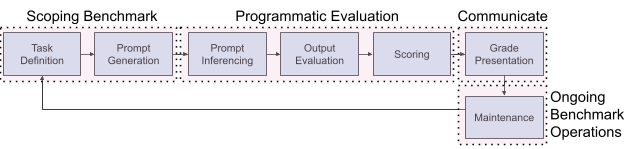
\includegraphics[width=0.9\textwidth]{image1.png}
  \caption{The chain of benchmark and assessment production follows a series of steps identified above.}
  \label{fig:benchmark-production}
\end{figure}

{\bf Step 1. Task Definition.} At this stage the benchmarking organization defines the task that the LLM is expected to perform and the desirable (or undesirable) behaviors against which it is being measured. Risk \#001, which indicates there is a disconnect between the user's understanding of the benchmark and what the benchmark is actually measuring is a risk to the intelligibility of the benchmark. This categorization implies a critique of many common benchmarks that cover a vast array of capabilities without a definite scope to the benchmark. Such benchmarks greatly advance the capabilities of LLMs through their generality, but they do not provide a means for forming a mental model of what the benchmark is indicating. Analogously, the user may know an engine's horsepower, but not know whether it is in a car or a boat.

\begin{center}
    \begin{tcolorbox}[colback=gray!10, colframe=black!50, width=\textwidth, boxrule=0.5mm, sharp corners, coltext=black]
        {\bf Example Risk:} \#001
        \newline
        {\bf Description:} ``Specified task does not match task performed for user"
    \end{tcolorbox}
\end{center}

{\bf Step 2. Prompt Generation.} Having defined the task the LLM is expected to perform, the next step is to produce data related to that task. Since many LLM developers work with publicly available internet data, one major risk to the correctness of a benchmark is that the benchmark uses publicly available data that is in the training set of the model. Worse yet, data vendors providing prompts consistent with a testing specification may charge the benchmarking organization for data that is publicly available and part of the training program for the benchmarked systems. This particular risk can be mitigated by searching for a select sample of test data within common datasets (e.g., \cite{commoncrawl}).

\begin{center}
    \begin{tcolorbox}[colback=gray!10, colframe=black!50, width=\textwidth, boxrule=0.5mm, sharp corners, coltext=black]
        {\bf Example Risk:} \#003
        \newline
        {\bf Description:} ``Prompts are collected from publicly available sources and presented as novel"
    \end{tcolorbox}
\end{center}

{\bf Step 3. Prompt Inferencing.} After producing the benchmark dataset, it is time to pipe the data through systems under test (SUTs) to get the outputs. Since many popular LLMs are closely guarded by their companies and only run for users on company-controlled hardware, benchmark prompts are often sent to SUT developers via their public APIs. If the SUT developer then accidentally or intentionally logs the prompts and brings them into their model engineering, the benchmark will no longer be reliable. The risk that the prompts will be exposed to one or more SUT developers is then the sum of the risks expressed across all benchmarked SUTs. Thus a benchmark that only benchmarks SUTs on the benchmark organization's hardware is more reliable, but likely less useful as the most important SUTs to relying persons are likely not to be covered.

\begin{center}
    \begin{tcolorbox}[colback=gray!10, colframe=black!50, width=\textwidth, boxrule=0.5mm, sharp corners, coltext=black]
        {\bf Example Risk:} \#020
        \newline
        {\bf Description:} ``Prompts are sent to model vendors when inferencing"
    \end{tcolorbox}
\end{center}

{\bf Step 4. Output Evaluation.} After inference the benchmark dataset, the SUT outputs are typically high dimensional (e.g., full text) and require interpretation consistent with the benchmark's purpose. Often this task is performed by an evaluator model, such as an LLM. Imagine now that an open source LLM is applied for this purpose. Any SUT developer could then place the evaluator LLM into its system chain to achieve a perfect score on the benchmark. Two mitigations are possible for this particular risk. Either the evaluator model can be kept strictly internal to the benchmark evaluation, or the machine evaluator could be replaced entirely by human effort.

\begin{center}
    \begin{tcolorbox}[colback=gray!10, colframe=black!50, width=\textwidth, boxrule=0.5mm, sharp corners, coltext=black]
        {\bf Example Risk:} \#023
        \newline
        {\bf Description:} ``SUT developers place evaluator within system chain"
    \end{tcolorbox}
\end{center}

{\bf Step 5. Scoring.} Having labeled each individual SUT output, the next step is to statistically aggregate the mitigations so they can be presented to the user in some form. One example risk at this step is that important relationships uncovered at the sample level might be hidden in the aggregate. A SUT for English, French, and Hindi might perform well for English and French, while failing spectacularly for Hindi. If the scoring function produces a simple average without propagating the Hindi failure, then the benchmark is not reliable for Hindi use decisions. Such problems can be mitigated by propagating uncertainty, confidence, and exceptions as a data structure to the presentation step.

\begin{center}
    \begin{tcolorbox}[colback=gray!10, colframe=black!50, width=\textwidth, boxrule=0.5mm, sharp corners, coltext=black]
        {\bf Example Risk:} \#029
        \newline
        {\bf Description:} ``Failure to propagate uncertainty or confidence from lower level measures to higher level grades"
    \end{tcolorbox}
\end{center}

{\bf Step 6. Grade Presentation.} At the presentation step, the benchmark score is rendered for consumption by the user. The most common presentation at the moment is HuggingFace.co leaderboards, which are typically up to date with the latest LLM releases. Few benchmarks are fully detailed on the HuggingFace platform (e.g., contextualizing each score with information on uncertainty). They also often lack information on what not to rely on the benchmark for. As such, there is a risk the user will not understand the scope of the benchmark as presented and make a false assumption of what an LLM may appropriately be asked to do.

\begin{center}
    \begin{tcolorbox}[colback=gray!10, colframe=black!50, width=\textwidth, boxrule=0.5mm, sharp corners, coltext=black]
        {\bf Example Risk:} \#033
        \newline
        {\bf Description:} ``User misunderstands the scope of the benchmark"
    \end{tcolorbox}
\end{center}

{\bf Step 7. Upkeep.} The final step of the benchmark production cycle is upkeep. Benchmark organizations today typically deliver benchmarks and move on to the next problem, but LLMs and the world they act within are constantly changing. So too must the benchmarks. Setting aside the possibility of SUT developers gaming a benchmark to achieve unrealistic scores, users themselves change in their capacities, use cases, and environments. Work establishing the ecological validity of a prompt set for processing current slang will become invalid within months as new words are introduced into prompts.

\begin{center}
    \begin{tcolorbox}[colback=gray!10, colframe=black!50, width=\textwidth, boxrule=0.5mm, sharp corners, coltext=black]
        {\bf Example Risk:} \#036
        \newline
        {\bf Description:} ``User behavior shifts through time"
    \end{tcolorbox}
\end{center}
